\documentclass{beamer}
\usepackage{tikz}

\usepackage{graphicx}
\usepackage[spanish]{datetime2}
\usepackage[spanish]{babel}
\usepackage{hhline}
\usepackage{epstopdf}
\usepackage{diagbox}
\usepackage{subcaption}
\usepackage{svg}
\usepackage{hyperref}


\usetheme{Madrid}
\definecolor{blmblue}{HTML}{003366}  % Granate UDC d2007b
\setbeamercolor{structure}{fg=blmblue} % Aplicar el color BLM a la estructura

\setbeamertemplate{navigation symbols}{}

\title[Trabajo Fin de Grado]{Perfilado automático de usuarios en corpus sociales sobre el movimiento \textit{Black Lives Matter}}
\author{Nicolás Míguez García}
\institute[GEI]{Grado en Ingeniería Informática (Mención en Computación) \\
	\vspace{3mm}
	Patricia Martín Rodilla \\ 
	David Otero Freijeiro 
} 

\date[\today]{}

\addtobeamertemplate{title page}{
	\begin{tikzpicture}[remember picture,overlay]
		\node[anchor=west,xshift=9pt,yshift=-8cm] at (current page.north west) {
\includegraphics[scale=0.05]{Logo_fic.jpg}}; 
		\node[anchor=east,xshift=-3.5pt,yshift=-8.5cm] at (current page.north east) {
\includegraphics[scale=0.12]{udc.png}};
	\end{tikzpicture}
}

\begin{document}
	
	\frame{\titlepage}
%	\begin{frame}
%	\end{frame}
		
	\AtBeginSection[]
	{
		\begin{frame}<beamer>
			\frametitle{Índice general}
			\tableofcontents[currentsection]
		\end{frame}
	}
\section{Introducción}

%\begin{frame}
%	\frametitle{Introducción}
%	\framesubtitle{\textit{Contexto}}
%			\begin{itemize}
%			\item El crecimeinto de 
%			\item Política.
%			\item Marketing.
%		\end{itemize}
%\end{frame}
		\begin{frame}
			\frametitle{Introducción}
			\framesubtitle{\textit{Author profiling}}
			El \textbf{\textit{author profiling}} consiste en el uso del NLP y aprendizaje automático para la extracción automática de características de autores de textos. \pause
			Permite el análisis masivo de datos de redes sociales para:\pause
			\begin{itemize}
				\item Investigación sociológica.
				\item Política.
				\item Marketing.
			\end{itemize}
		\end{frame}
		
		\begin{frame}
			\frametitle{Objetivos}
			\begin{itemize}
				\item Estudio del \textbf{estado del arte} del \textit{author profiling} en materia de género y edad sobre textos en {español}.
				\item {Reproducción de los \textbf{algoritmos}} con mejor rendimiento.
				\item Construcción de una \textbf{herramienta} para el análisis de grandes conjuntos de usuarios.
				\item Estudio de \textbf{resultados} de perfilado sobre colección...
			\end{itemize}
		\end{frame}
		
\section{Fundamentos}
		\subsection{Estado del arte}
		\begin{frame}
			\frametitle{Fundamentos}
			\framesubtitle{Estado del arte}
			\begin{itemize}
				\item Trabajos tempranos sobre blogs (2006 y 2007). \pause
				\item Competiciones PAN a partir de 2013. \pause
				\item IberLEF 2022.\pause
				\item Recursos limitados en idioma español.\pause
			\end{itemize}
		\end{frame}
%		\subsection{Cojuntos de datos}
%		\begin{frame}
%			\frametitle{Fundamentos}
%			\framesubtitle{Conjuntos de datos}
%			\begin{table}[hp!]
%				\centering
%				\begin{tabular}{|l|ll|l|l|}
%					\hhline{~---~}
%					\multicolumn{1}{c|}{} & \multicolumn{2}{c|}{\textbf{PAN-AP 2015}} & \textbf{PAN-AP 2016} & \multicolumn{1}{c}{}\\ \hline
%					Categoría & Training & Test & Training & Total\\ \hline
%					18-24 & 22 & 18 & 11 & 51\\
%					25-34 & 46 & 44 & 54 & 144\\
%					35-49 & 22 & 18 & 116 & 156\\
%					+50 & 10 & 8 & 41 & 59\\ \hline
%					Hombres & 50 & 44 & 111 & 204\\
%					Mujeres & 50 & 44 & 111 & 204\\ \hline
%					Total & 100 & 88 & 222 & 410\\ \hline  
%				\end{tabular}%
%				\caption{Distribución de usuarios en función de edad y género en los conjuntos de entrenamiento utilizados.}
%				\label{tab:datasets_edad}
%			\end{table}
%		\end{frame}
		
%		\begin{frame}
%			\frametitle{Algoritmos de perfilado}
%			\framesubtitle{1ª aproximación}
%			\begin{itemize}
%				\item Ganador IberLef 2022 (ideología política).
%				\item  Red neuronal basada en \textit{transformers}.
%				\item \textit{Embeddings} de BETO y MarIA.
%				\item Entrenamiento y uso costosos (TPU).
%				\item Peor rendimiento de los tres.
%				\item Requiere + datos de entrenamiento.
%
%			\end{itemize}
%		\end{frame}
%		
%		\begin{frame}
%			\frametitle{Algoritmos de perfilado}
%			\framesubtitle{2ª aproximación}
%			\begin{itemize}
%				\item 3º en PAN 2015 (personalidad).
%				\item Máquina de soporte vectorial.
%				\item Tf-idf n-gramas de 3 caracteres.
%				\item El mejor en edad.
%			\end{itemize}
%		\end{frame}
%		
%		\begin{frame}
%			\frametitle{Algoritmos de perfilado}
%			\framesubtitle{3ª aproximación}
%			\begin{itemize}
%				\item 2º en PAN 2016 (multi-género).
%				\item Regresión logística.
%				\item Tf-idf n-gramas distintos rangos.
%				\item \textit{Features} estilísticas (puntuación y ortografía)
%				\item Mejor en clasificación de género.
%			\end{itemize}
%		\end{frame}
%		
%		\begin{frame}
%			\frametitle{Algoritmos de perfilado}
%			
%			\begin{table}[H]
%				\centering
%				{
%					\setlength{\tabcolsep}{0.3\tabcolsep}
%					\begin{tabular}{|l|ll|ll|}
%						\hhline{~----}
%						\multicolumn{1}{c}{} &  \multicolumn{2}{|c|}{\textbf{Género}} & \multicolumn{2}{c|}{\textbf{Edad}} \\ \hline
%						\textbf{Aprox} & \textbf{Acc} & \textbf{F1-w} & \textbf{Acc} & \textbf{F1-w}\\ \hline
%						
%						2ª  & 0.7024 & 0.6960 & 0.6073  & \textbf{0.5657} \\
%						3ª  & \textbf{0.8120} & \textbf{0.8193} & \textbf{0.6423} & 0.5611 \\ \hline
%						
%					\end{tabular}
%				}
%				\caption{Tabla comparativa con los resultados de las tres aproximaciones seleccionadas.}
%				\label{tab:fundamentos-comparativa}
%			\end{table}
%			
%		\end{frame}
		\subsection{Algoritmos de perfilado}
		\begin{frame}
			\frametitle{Fundamentos}
			\framesubtitle{Algoritmos de perfilado}
			Se seleccionaron 3 algoritmos:
			\begin{columns}[T]
				\hspace{-3cm}
				\begin{column}{0.8\textwidth}
					\begin{description}[labelwidth=0.01mm]
						\item \textbf{1º Carrasco y Rosillo} 
								\begin{itemize}
									\item 1º IberLEF 2022.\pause
									\item Más prometedor.\pause
									\item Peor rendimiento de los tres.\pause
									\item No se ha terminado usando.\pause

								\end{itemize}
						\vspace{0.8cm} \pause
						\item \textbf{2º Grivas:} 
							\begin{itemize}
								\item 3º en AP-PAN 2015.\pause
								\item El mejor en edad.\pause
							\end{itemize}
					\end{description}
				\end{column}
				\hspace{-3.5cm}
				\begin{column}{0.8\textwidth}
					\begin{description}[labelwidth=0.01mm] \pause
						\item \textbf{3ª Modaresi:} 
						\begin{itemize}
							\item 2º en PAN 2016.\pause
							\item Independencia del género escritura.\pause
							\item Mejor en clasificación de género usuarios.\pause
						\end{itemize}
%						\vspace{0.35cm} 
%%						\item \textbf{Elección del XGBoost:} 
%
%							\begin{table}[H]
%								\centering
%									\resizebox{0.5\textwidth}{!}{%{
%										\setlength{\tabcolsep}{0.3\tabcolsep}
%										\begin{tabular}{|l|ll|ll|}
%											\hhline{~----}
%											\multicolumn{1}{c}{} &  \multicolumn{2}{|c|}{\textbf{Género}} & \multicolumn{2}{c|}{\textbf{Edad}} \\ \hline
%											\textbf{Aprox} & \textbf{Acc} & \textbf{F1-w} & \textbf{Acc} & \textbf{F1-w}\\ \hline
%											
%											2ª  & 0.7024 & 0.6960 & 0.6073  & \textbf{0.5657} \\
%											3ª  & \textbf{0.8120} & \textbf{0.8193} & \textbf{0.6423} & 0.5611 \\ \hline
%											
%										\end{tabular}
%									}%
%								\label{tab:fundamentos-comparativa}
%							\end{table}
					\end{description}
				\end{column}
			\end{columns}
		\end{frame}
\section{Fenómeno \#BLM}
\subsection{Contexto movimiento}
\begin{frame}
	\frametitle{Colección de estudio}
	\framesubtitle{\textit{Black Lives Matter}}
	
	\begin{columns}[T] % La opción [T] alinea la parte superior de las columnas
		\begin{column}{0.5\textwidth}
			
\includegraphics[width=\textwidth]{blm}
		\end{column}
		\begin{column}{0.5\textwidth}
			\pause
			Varios investigadores construyeron una colección para el estudio de este movimiento:
			\begin{itemize}
				\item Un año de actividad.
				\item +260.000 publicaciones de +90.000 usuarios.
				\item Inglés y español.
			\end{itemize}
		\end{column}
	\end{columns}
\end{frame}
\subsection{Demo}
\begin{frame}
\frametitle{Demo}

\begin{center}
	\href{run://usr/bin/vlc final.mp4}{
		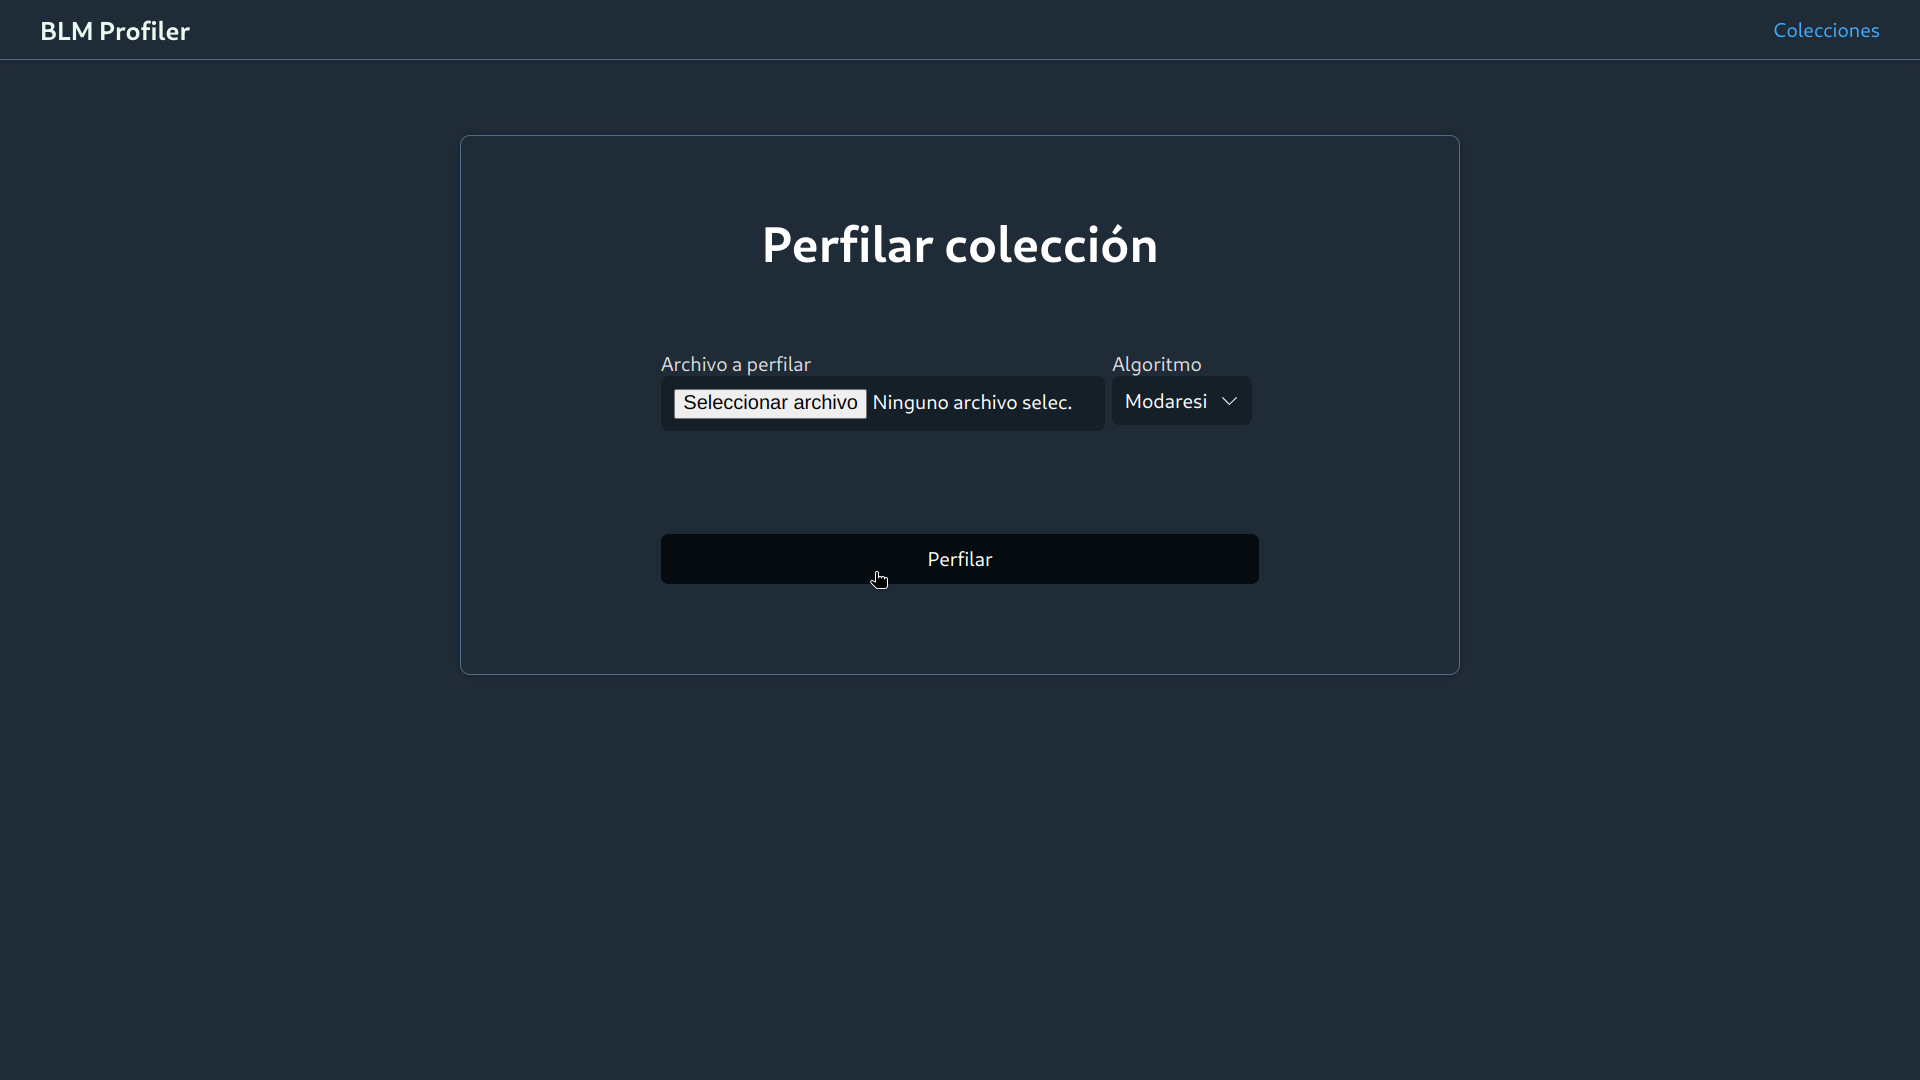
\includegraphics[width=0.5\textwidth]
		{final.png}}
\end{center}
	
\end{frame}
\subsection{Análisis resultados}

% \begin{frame}
	%	\frametitle{Resultados perfilado}
	%	\framesubtitle{Algorimto de Modaresi - Edad}
	% \begin{figure}[H]
		%	\centering
		%	\begin{subfigure}{0.2\textwidth}
			%		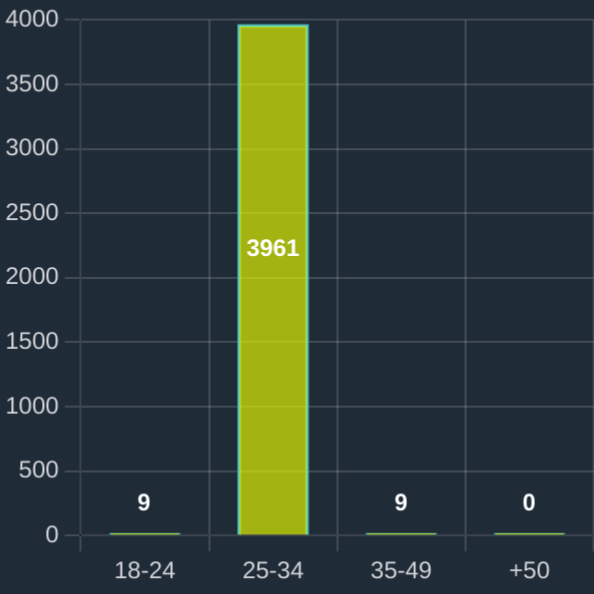
\includegraphics[width=\textwidth]{imaxes/capturas-app/graficos/modaresi/grafico-edad-moda.png}
			%		\caption{Total}
			%		\label{subfig:blm/resultados-edad-moda}
			%	\end{subfigure}
		%	\begin{subfigure}{0.2\textwidth}
			%		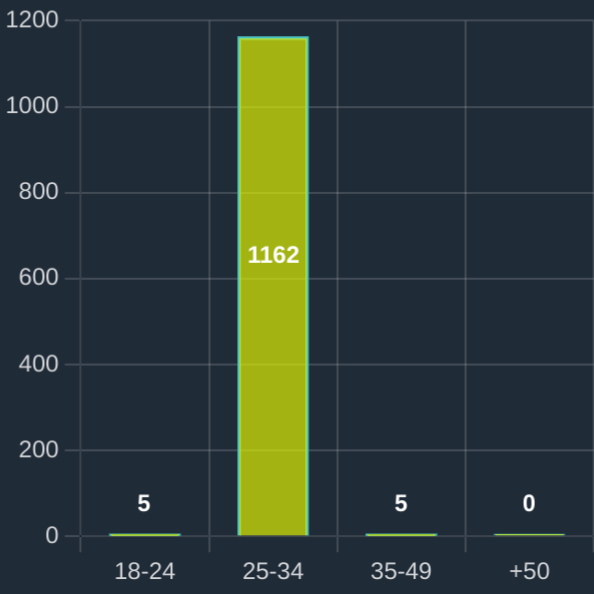
\includegraphics[width=\textwidth]{imaxes/capturas-app/graficos/modaresi/grafico-edad-moda-fem.png}
			%		\caption{Usuarios femeninos} 
			%	\end{subfigure}
		%	\begin{subfigure}{0.18\textwidth}
			%		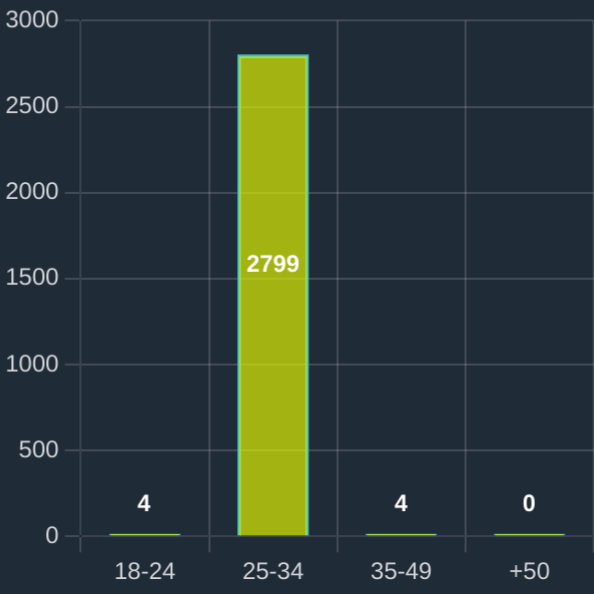
\includegraphics[width=\textwidth]{imaxes/capturas-app/graficos/modaresi/grafico-edad-moda-masc.png}
			%		\caption{Usuarios masculinos} 
			%	\end{subfigure}
		% \end{figure}
	%	\begin{figure}[H]
		%	\begin{subfigure}{0.18\textwidth}
			%		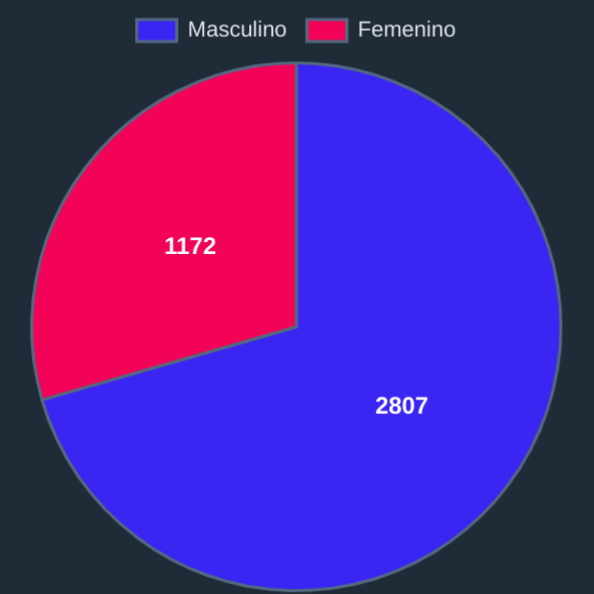
\includegraphics[width=\textwidth]{imaxes/capturas-app/graficos/modaresi/grafico-genero.png}
			%		\caption{Total}
			%		\label{subfig:blm/resultados-genero-moda}
			%	\end{subfigure}
		%	\begin{subfigure}{0.18\textwidth}
			%		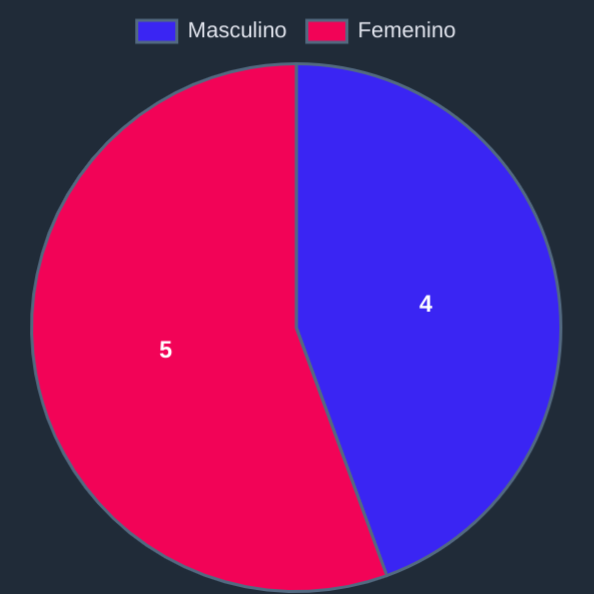
\includegraphics[width=\textwidth]{imaxes/capturas-app/graficos/modaresi/grafico-genero-jj.png}
			%		\caption{18-24 años}
			%	\end{subfigure}
		%	\begin{subfigure}{0.18\textwidth}
			%		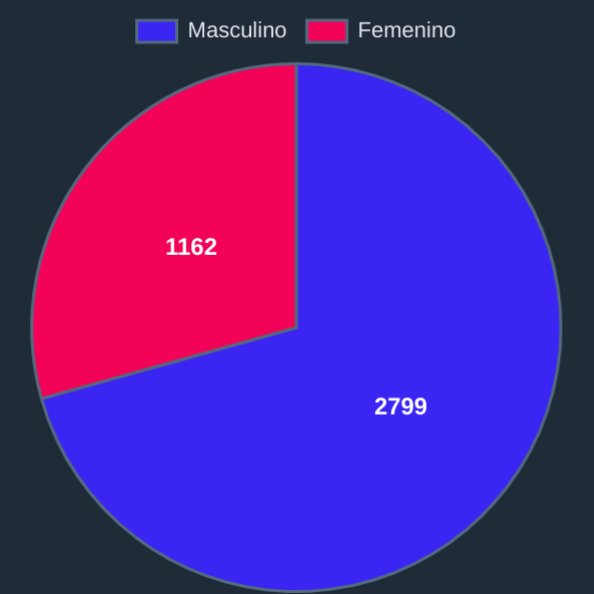
\includegraphics[width=\textwidth]{imaxes/capturas-app/graficos/modaresi/grafico-genero-j.png}
			%		\caption{25-34 años}
			%	\end{subfigure}
		%	\begin{subfigure}{0.18\textwidth}
			%		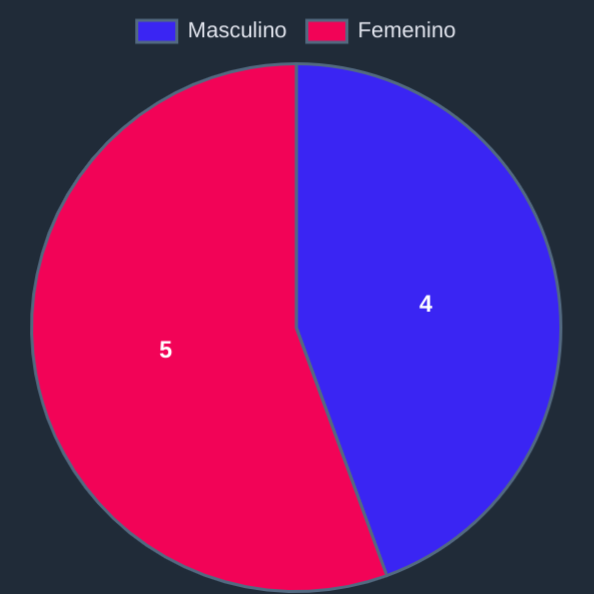
\includegraphics[width=\textwidth]{imaxes/capturas-app/graficos/modaresi/grafico-genero-v.png}
			%		\caption{35-49 años}
			%	\end{subfigure}
		%	\begin{subfigure}{0.18\textwidth}
			%		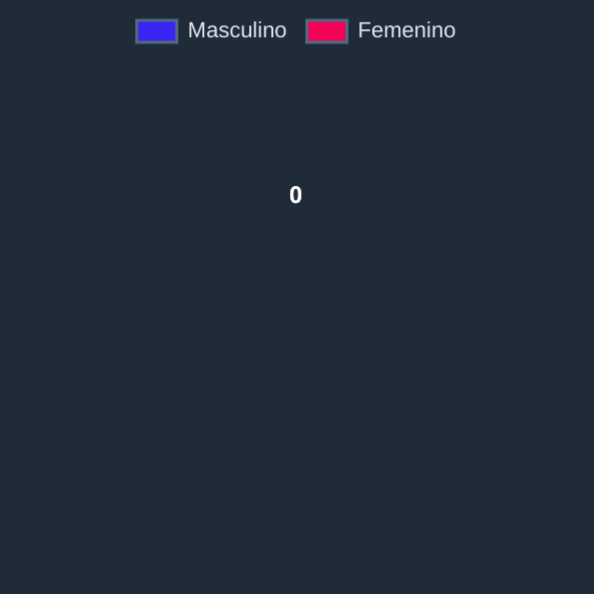
\includegraphics[width=\textwidth]{imaxes/capturas-app/graficos/modaresi/grafico-genero-vv.png}
			%		\caption{+50 años}
			%	\end{subfigure}
		% \end{figure}
	
	% \end{frame}


\begin{frame}
	\frametitle{Resultados perfilado}
	\framesubtitle{Algoritmo de Grivas}
	\begin{figure}[H]
		\centering
		\begin{subfigure}{0.3\textwidth}
			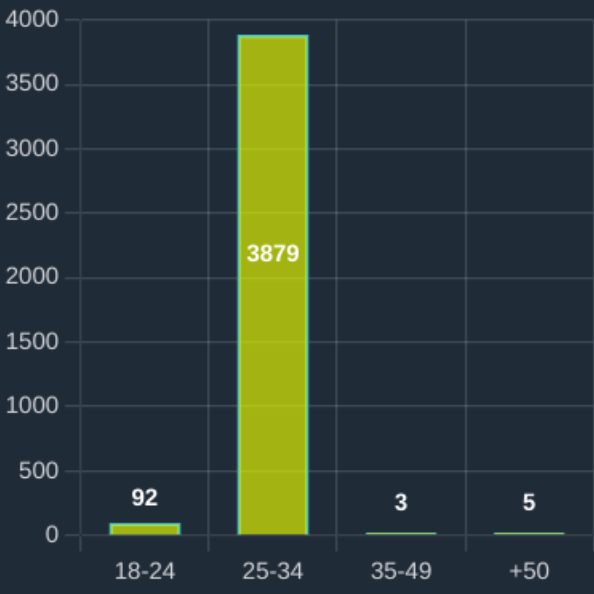
\includegraphics[width=\textwidth]{imaxes/capturas-app/graficos/grivas/grafico-edad-grivas.png}
			\caption{Edad}
			\label{subfig:blm/resultados-edad-moda}
		\end{subfigure}
		\begin{subfigure}{0.3\textwidth}
			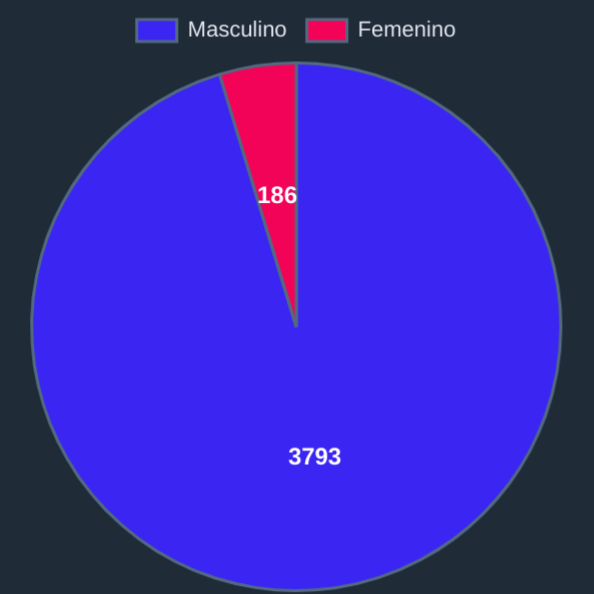
\includegraphics[width=\textwidth]{imaxes/capturas-app/graficos/grivas/grafico-genero.png}
			\caption{Género}
			\label{subfig:blm/resultados-genero-moda}
		\end{subfigure}
	\end{figure}
	\begin{table}[H]
		{
			\setlength{\tabcolsep}{0.6\tabcolsep}
			\begin{tabular}{|c|c|c|c|c|c|}
				\hline
				\diagbox{\textbf{Género}}{\textbf{Edad}} & \textbf{18-24} & \textbf{25-34} & \textbf{35-49} & \textbf{+50} & \textbf{Total} \\ \hline
				\textbf{Femenino} & 31 & 154 & 0 & 1 & 186 \\ \hline
				\textbf{Masculino} & 61 & 3725 & 3 & 4 & 3793 \\ \hline
				\textbf{Total} & 92 & 3879 & 3 & 5 & 3979 \\ \hline
				
			\end{tabular}%
		}
	\end{table}
\end{frame}


\begin{frame}
	\frametitle{Resultados perfilado}
	\framesubtitle{Algoritmo de Modaresi}
	\begin{figure}[H]
		\centering
		\begin{subfigure}{0.3\textwidth}
			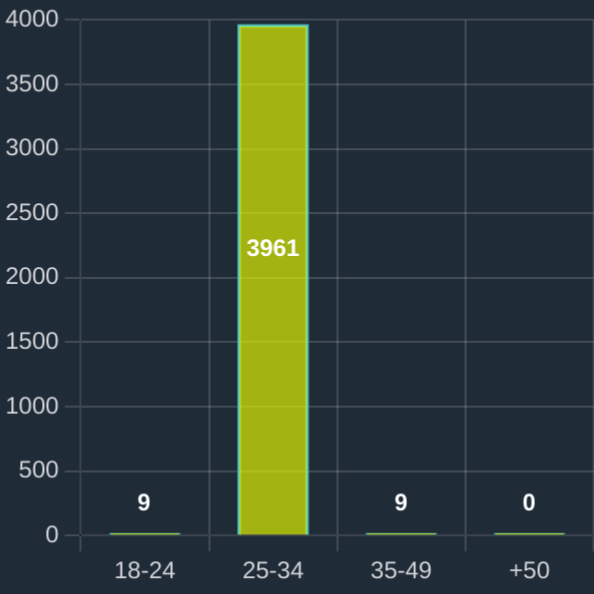
\includegraphics[width=\textwidth]{imaxes/capturas-app/graficos/modaresi/grafico-edad-moda.png}
			\caption{Edad}
			\label{subfig:blm/resultados-edad-moda}
		\end{subfigure}
		\begin{subfigure}{0.3\textwidth}
			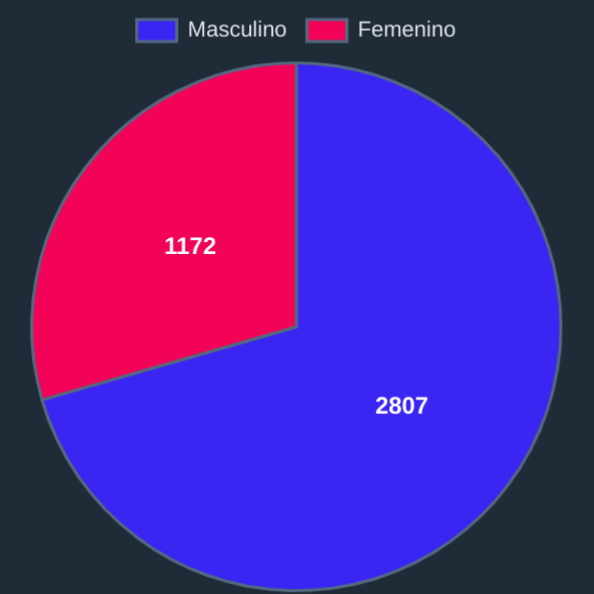
\includegraphics[width=\textwidth]{imaxes/capturas-app/graficos/modaresi/grafico-genero.png}
			\caption{Género}
			\label{subfig:blm/resultados-genero-moda}
		\end{subfigure}
	\end{figure}
	\begin{table}[H]
		\centering
		{
			\setlength{\tabcolsep}{0.6\tabcolsep}
			\begin{tabular}{|c|c|c|c|c|c|}
				\hline
				\diagbox{\textbf{Género}}{\textbf{Edad}} & \textbf{18-24} & \textbf{25-34} & \textbf{35-49} & \textbf{+50} & \textbf{Total} \\ \hline
				\textbf{Femenino} & 5 & 1162 & 5 & 0 & 1172 \\ \hline
				\textbf{Masculino} & 4 & 2799 & 4 & 0 & 2807 \\ \hline
				\textbf{Total} & 9 & 3961 & 9 & 0 & 3979 \\ \hline
				
			\end{tabular}%
		}
	\end{table}
\end{frame}


\begin{frame}
	\frametitle{Resultados perfilado}
	\framesubtitle{Discusión}
	\begin{columns}[T]
		\hspace{-3.5cm}
		\begin{column}{\textwidth}
			\begin{description}[labelwidth=0.01mm]
				\item 
				\begin{itemize}
					\item<1-> Grupo 25-34 años $>$ 95\% (desequilibrio entrenamiento)
					\item<3-> Usuarios masculinos $>$ 75\%.
					\item<4-> Distribución Reddit $\implies$ distribución corpus.
					\item<5-> 48.98\% $\rightarrow$ 1 publicación.\\
					 80\% $\rightarrow$ menos de 5.
					\\ \hspace{2cm}$\downarrow$
					\item <6-> Baja fiabilidad.
					\item <7-> Resultados similares inglés.
				\end{itemize}
			\end{description}
			
		\end{column}
		\hspace{-1.5cm}
		\onslide<2->{
			\hspace{-2.5cm}
			\begin{column}{0.6\textwidth}
 			\begin{description}[labelwidth=0.01mm]
					\item

				\vspace{-0.75cm}
				\begin{figure}[H]
					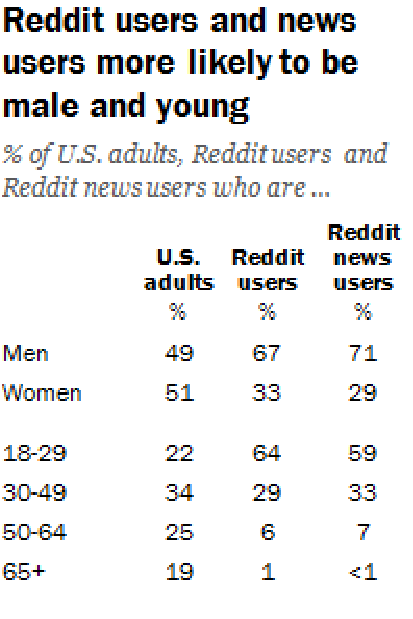
\includegraphics[width=0.5\textwidth]{imaxes/estudio-reddit.pdf}
				\end{figure}
				{\tiny Fuente: Pew Research Center (estudio 2016 ).}
				\end{description}

		\end{column}}
	\end{columns}
\end{frame}


\section{Metodología y gestión del proyecto}
 \begin{frame}
 	
 	\frametitle{Metodología}
 	\framesubtitle{Elección y adaptaciones}

 		\begin{columns}[T]
 		\hspace{-3cm}

 		\begin{column}{0.8\textwidth}
 			\begin{description}[labelwidth=0.01mm]
				\item \textbf{Consideraciones proyecto}
			 	\begin{itemize}
				\item Carácter innovador.
				\item Falta recursos español.
				\item Escaso conocimiento.
			 	\end{itemize}
			 	\pause
 				\hspace{3cm}$\downarrow$ \\
		 		\textbf{Scrum}
	 	 		\begin{itemize}
			 	 	\item Metodología ágil.
			 		\item Transparencia, inspección y adaptación.
		 		\end{itemize}
			\end{description}
		 \end{column}
	 	\pause
	 	\hspace{-3.5cm}
		 \begin{column}{0.8\textwidth}
		 	\begin{description}[labelwidth=0.01mm]
		 		\item \textbf{Adaptaciones Scrum} 			 	\pause
		 		\begin{itemize}
		 			\item Roles
		 			\item Eventos
		 			\item Artefactos
%		 			\item  Product Owner $\rightarrow$ estudiante
%		 			\item Scrum master $\rightarrow$ directores
%		 			\item  Equipo de trabajo $\rightarrow$ estudiante \pause
%		 			\item \textit{Sprints} $\rightarrow$ 3 semanas
%		 			\item Carga de trabajo no uniforme	\pause
%		 			\item \textit{Daily review} $\rightarrow$ autovaloración
%		 			\item \textit{Product Backlog}: tareas técnicas e historias de usuario.
		 		\end{itemize}
		 	\end{description}
	 	\end{column}
	\end{columns}
\end{frame}
\begin{frame}
	\frametitle{Gestión del proyecto}
	\framesubtitle{Estimación y costes}
	\begin{itemize}
		\item 9 sprints en total. \pause
		\item Cada uno $\approx$ 45 horas de trabajo (3 h/día). \pause
		\item Recursos humanos: alumno (18€/h) y directores (31€/h).\pause
		\item Ordenador portátil $\approx$ 428€.
	\end{itemize}
	\pause
	\vspace{1cm}
\textbf{	Cálculo final:}
	\begin{table}[H]
		\centering
		{
			\setlength{\tabcolsep}{1\tabcolsep}
			\begin{tabular}{|c|c|c|c|}
				\hline
				\textbf{Rol} & \textbf{Coste/hora} & \textbf{Tiempo de trabajo} & \textbf{Total} \\ \hline
				Equipo & 18€ & 45h x 9 \textit{sprints} & 7.290 € \\ \hline
				\textit{Project Managers} & 31€ & 2 x 1.5h x 9 \textit{sprints} & 837 € \\ \hline
				Material & -- & -- & 428 € \\ \hline
				\textbf{Total} & -- & -- & \textbf{8.555 €} \\ \hline
				
			\end{tabular}%
		}
%		\caption{Tabla con el cálculo de costes final para el proyecto.}
		\label{tab:metodologia/costes}
	\end{table}
	
	
\end{frame}
\section{Diseño}
	\begin{frame}
	\frametitle{Diseño}
	\framesubtitle{Arquitectura global}
	Se ha optado por una arquitectura cliente-servidor distribuida en 3 capas. \pause
	\begin{figure}[H]
		\centering
		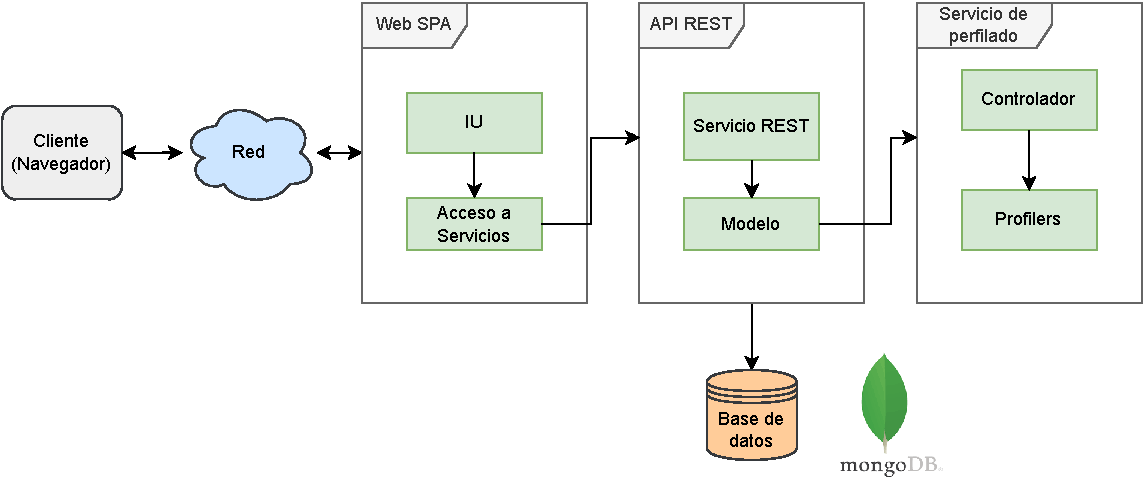
\includegraphics[width=\textwidth]{arquitectura.pdf}
		%			\caption{Diagrama de la arquitectura global del sistema.}
		\label{fig:diagrama/arquitectura}
	\end{figure}
\end{frame}


\section{Conclusiones}

	\begin{frame}
			\frametitle{Conclusiones}
			\framesubtitle{Evaluación estado actual y lecciones aprendidas}
			\vspace{0cm}
			\textbf{Resultados:}
			\begin{itemize}
				\item Varios algorimtos de perfilado.\pause
				\item Herramienta para el análisis de grandes colecciones.\pause
				\item Análisis movimiento \#BLM. 

			\end{itemize} 
			\pause
			\vspace{0.5cm}
			\textbf{Lecciones aprendidas:}  \pause
			\begin{itemize}
				\item Importancia organización metodológica. \pause
				\item Relación conocimientos. \pause
				\item Crecimiento personal.
			\end{itemize}
	\end{frame}
	
	\begin{frame}
		\frametitle{Trabajo futuro}
%		Dos líneas:

		\begin{columns}[T]
				\hspace{-3cm}
			\begin{column}{0.8\textwidth}
				\begin{description}[labelwidth=0.01mm]
					\item \textbf{Algoritmos perfilado:}
					\begin{itemize}
						\item Mejora corpus entrenamiento. \pause
						\item Nuevos modelos (LLM). \pause
						\item Aumento de atributos.
						\end{itemize}
				\end{description}
			\end{column}
				\hspace{-3cm}
			\begin{column}{0.8\textwidth}

				\begin{description}[labelwidth=0.01mm]
					\item \textbf{Funcionalidad aplicación:}
					\begin{itemize}
						\item Perfilado asíncrono. \pause
						\item Exportación de datos.\pause
						\item Explicación de predicción.
					\end{itemize}
				\end{description}
			\end{column}
		\end{columns}
	\end{frame}
	
\begin{frame}[plain]
	\begin{center}
		\Huge ¡Gracias por su atención!
	\end{center}
\end{frame}

\end{document}